\chapter{Formal Analysis} \label{alloy}

\section{Alloy code}

This section provides all the alloy code used to prove the correctness of the project. For a better reading, the code is subdivided into the different blocks it's composed.

\subsection{Entities}

\begin{minted}{Alloy}
// +--------------------------------------------+
// |                  General                   |
// +--------------------------------------------+

// Email address
sig Email {}

// Password
sig Password {}

// Booleans
abstract sig Boolean {}
lone sig True extends Boolean {}
lone sig False extends Boolean {}

// Date time, represented as an integer
sig DateTime {
    time: one Int
} {
    time >= 0
}

// Global time
lone sig GlobalTime {
    time: one DateTime
}

// +--------------------------------------------+
// |                   Common                   |
// +--------------------------------------------+

// eMSP user's vehicle
sig Vehicle {
    socket: one Socket,
    certificate: one Certificate
}


// Vehicle certificate
sig Certificate {}

// Sockets
abstract sig Socket {}
lone sig SocketSlow extends Socket {}
lone sig SocketFast extends Socket {}
lone sig SocketRapid extends Socket {}

// eMSP user's booking
sig Booking {
    chargingColumn: one ChargingColumn,
    start: one DateTime,
    end: one DateTime,
    vehicle: one Vehicle,
    user: one eMSPuser
} {
    start.time < end.time
}

// +--------------------------------------------+
// |                    eMSP                    |
// +--------------------------------------------+

// eMSP user
sig eMSPuser {
    username: one Email,
    password: one Password,
    devices: set Device,
    vehicles: set Vehicle,
    favorites: set ChargingStation
}

// eMSP user's device
sig Device {}

// +--------------------------------------------+
// |                    CPMS                    |
// +--------------------------------------------+

// CPMS
sig CPMS {
    users: set CPMSuser,
    chargingStations: some ChargingStation,
    bookings: set Booking
}

// CPMS user
sig CPMSuser {
    username: one Email,
    password: one Password,
    cpms: one CPMS,
    CSManaged: some ChargingStation
}






// CPO's charging station
sig ChargingStation {
    location: one Location,
    chargingColumns: some ChargingColumn,
    mix: one EnergyMix,
    dso: one DSO,
    availableDSOs: some DSO,
    automaticDsoChoice: some Boolean
} {
    dso in availableDSOs
}

// Charging station's column
sig ChargingColumn {
    chargingStation: one ChargingStation,
    socket: one Socket,
    occupied: one Boolean
}

// Location
sig Location {}

// CPMS energy mix
sig EnergyMix {}

// DSO
sig DSO {
    price: one Int
} {
    price > 0
}

// Energy source
abstract sig EnergySource {
    chargingStation: one ChargingStation,
    isBeingUsed: one Boolean
}

// Battery as the energy source
sig Battery extends EnergySource {
    chargeLevel: one Int,
    isCharging: one Boolean
} {
    chargeLevel >= 0 and chargeLevel <= 100
}

// Solar panel as the energy source
sig SolarPanel extends EnergySource {}

// DSO as the energy source
sig DSOenergy extends EnergySource {
    DsoUsed: one DSO
}
\end{minted}

\pagebreak

\subsection{Facts}

\begin{minted}{Alloy}
// +--------------------------------------------+
// |                   Common                   |
// +--------------------------------------------+

// Every email address has an owner
fact OwnedEmail {
    all e: Email | (
        (one u: eMSPuser | u.username = e)
        or
        (one u: CPMSuser | u.username = e)
    )
}

// No two distict eMSPusers or CPMSusers have the same username (email address)
fact OneUsername {
    (no disj u1, u2: eMSPuser | u1.username = u2.username)
    and
    (no disj u1, u2: CPMSuser | u1.username = u2.username)
}

// Every password is associated with at least one user
fact OwnPassword {
    all p: Password | (
        (some u: eMSPuser | u.password = p)
        or
        (some u: CPMSuser | u.password = p)
    )
}

// Every date time is used in a booking or is the global time
fact SomeDateTime {
    all d: DateTime |
        (some b: Booking |
            b.start = d
            or
            b.end = d)
        or
            d.time = Now[]
}

// No two date time represent share time
fact NoCommonTime {
    all d: DateTime |
        all d1: DateTime |
            d.time = d1.time
            implies
            d = d1
}

// Every socket is used somewhere
fact SocketUsed {
    all s: Socket | (
        (some cc: ChargingColumn | cc.socket = s)
        or
        (some v: Vehicle | v.socket = s)
    )
}


// +--------------------------------------------+
// |                    eMSP                    |
// +--------------------------------------------+

// Every device has only one owner
fact OwnedDevice {
    all d: Device |
        one u: eMSPuser |
            d in u.devices
}

// Every vehicle has only one owner
fact EveryVehicleIsOwned {
    all v: Vehicle |
        one u: eMSPuser |
            v in u.vehicles
}

// Every certificate is associated with only one vehicle
fact OneCertificateOneVehicle {
    all c: Certificate |
        one v: Vehicle |
            c = v.certificate
}

// +--------------------------------------------+
// |                    CPMS                    |
// +--------------------------------------------+

// Every charging station is associated to a CPMS
fact OneChargingStationOneCPMS {
    all cs: ChargingStation |
        one cpms: CPMS |
            cs in cpms.chargingStations
}

// Charging stations managed by a CPMS user are owned by that CPMS
fact ChargingStationCPMS{
    all u: CPMSuser |
        u.CSManaged & u.cpms.chargingStations = u.CSManaged
}

// Every location is associated with only one charging station
fact OneLocationOneChargingStation {
    all l: Location |
        one c: ChargingStation |
            c.location = l
}

// A charging column is associated with only one charging station
fact ChargingColumnOneStation {
    no disj c1, c2: ChargingStation |
        some cc: ChargingColumn |
            cc in (c1.chargingColumns & c2.chargingColumns)
}





// The charging column's station contains that column
fact ChargingStationColumn {
    all c: ChargingColumn |
        c in c.chargingStation.chargingColumns
}

// No battery can be still charging if its level is 100%
fact ChargingBattery {
    all b: Battery |
        b.isCharging = True
        implies
        b.chargeLevel < 100
}

// If automatic DSO choice is enabled, the DSO with the lowest price is selected
fact AutomaticDsoChoice {
    all cs: ChargingStation |
        cs.automaticDsoChoice = True
        implies
        all d: DSO |
            d in cs.availableDSOs
            implies
            cs.dso.price <= d.price
}

// Every DSO has to be associated with at least one charging station
fact OneDSOOneOrMoreChargingStation {
    all d: DSO |
        some c: ChargingStation |
            c.availableDSOs & d = d
}

// Every energy mix has to be associated with one charging station
fact OneEnergyMixOneChargingStation {
    all e: EnergyMix |
        some c: ChargingStation |
            c.mix = e
}

// A DSO energy associated to a charging station uses the dso used by that station
fact DSOUsed {
    all cs: ChargingStation, d: DSOenergy |
        d.chargingStation = cs
        implies
        d.DsoUsed = cs.dso
}

// All charging stations have a DSO energy
fact ExactlyDSOEnergyPerChargingStation {
    all cs: ChargingStation |
        one d: DSOenergy | d.chargingStation = cs
}








// All charging station have some energy sources that are being used
fact ActiveSourcesPerStation {
    all cs: ChargingStation |
        some e: EnergySource | 
            e.chargingStation = cs
            and
            e.isBeingUsed = True
}

// +--------------------------------------------+
// |                  Bookings                  |
// +--------------------------------------------+

// Every booking is associated to a CPMS
fact BookingCPMS {
    all b: Booking |
        one c: CPMS |
            b in c.bookings
}

// Every booking is associated to a charging column managed by the CPMS
fact BookingRightCPMSassociation {
    all b: Booking, c: CPMS |
        b in c.bookings
        implies
        b.chargingColumn.chargingStation in c.chargingStations
}

// The same column can't have two overlapping bookings
fact BookNoOverlapOnColumn {
    all disj b1, b2: Booking |
        b1.chargingColumn = b2.chargingColumn 
        implies
        b1.start.time > b2.end.time or b2.start.time > b1.end.time 
}

// The same vehicle can't have two overlapping bookings
fact BookNoOverlapOnVehicle {
    all disj b1, b2: Booking |
        b1.vehicle = b2.vehicle
        implies
        b1.start.time > b2.end.time or b2.start.time > b1.end.time
}

// The user has to book a column that is compatible with the vehicle's socket
fact BookedRightColumn {
    all b: Booking |
        b.chargingColumn.socket = b.vehicle.socket
}

// For every booked charge, the vehicle is owned by the user who booked
fact BookedChargeVehicleOwner {
    all b: Booking |
        b.vehicle in b.user.vehicles
}





// If a charging column is occupied, there exists a booking that occupies it at the given
// global time
fact ChargingColumnOccupied {
    all c: ChargingColumn |
        c.occupied = True
        implies
        one b: Booking |
            b.chargingColumn = c
            and
            b.start.time <= Now[]
            and
            b.end.time >= Now[]
}
\end{minted}

\subsection{Functions}

\begin{minted}{Alloy}
fun Now[]: Int {
    GlobalTime.time.time
}
\end{minted}

\pagebreak

\section{Alloy generated worlds}

Here there are some generated worlds from the alloys source that show some functionalities of the system. Each one of them has a brief description of the depicted situation, the predicate used for showing it, and the generated diagram.

\subsection{Ongoing charge of a vehicle}

This diagram shows the charging process of a vehicle, pointing out the occupation of that charging column by the user's vehicle, while the other one is free.

\begin{minted}{Alloy}
pred OngoingCharge {
    #Device = 1
    #eMSPuser = 1
    #CPMSuser = 0
    #Vehicle = 1
    #DSO <= 1
    #ChargingStation = 1
    #ChargingColumn = 2
    #Booking >= 2
    some c: ChargingColumn | c.occupied = True
}
\end{minted}

\begin{figure}[h!]
    \centering
    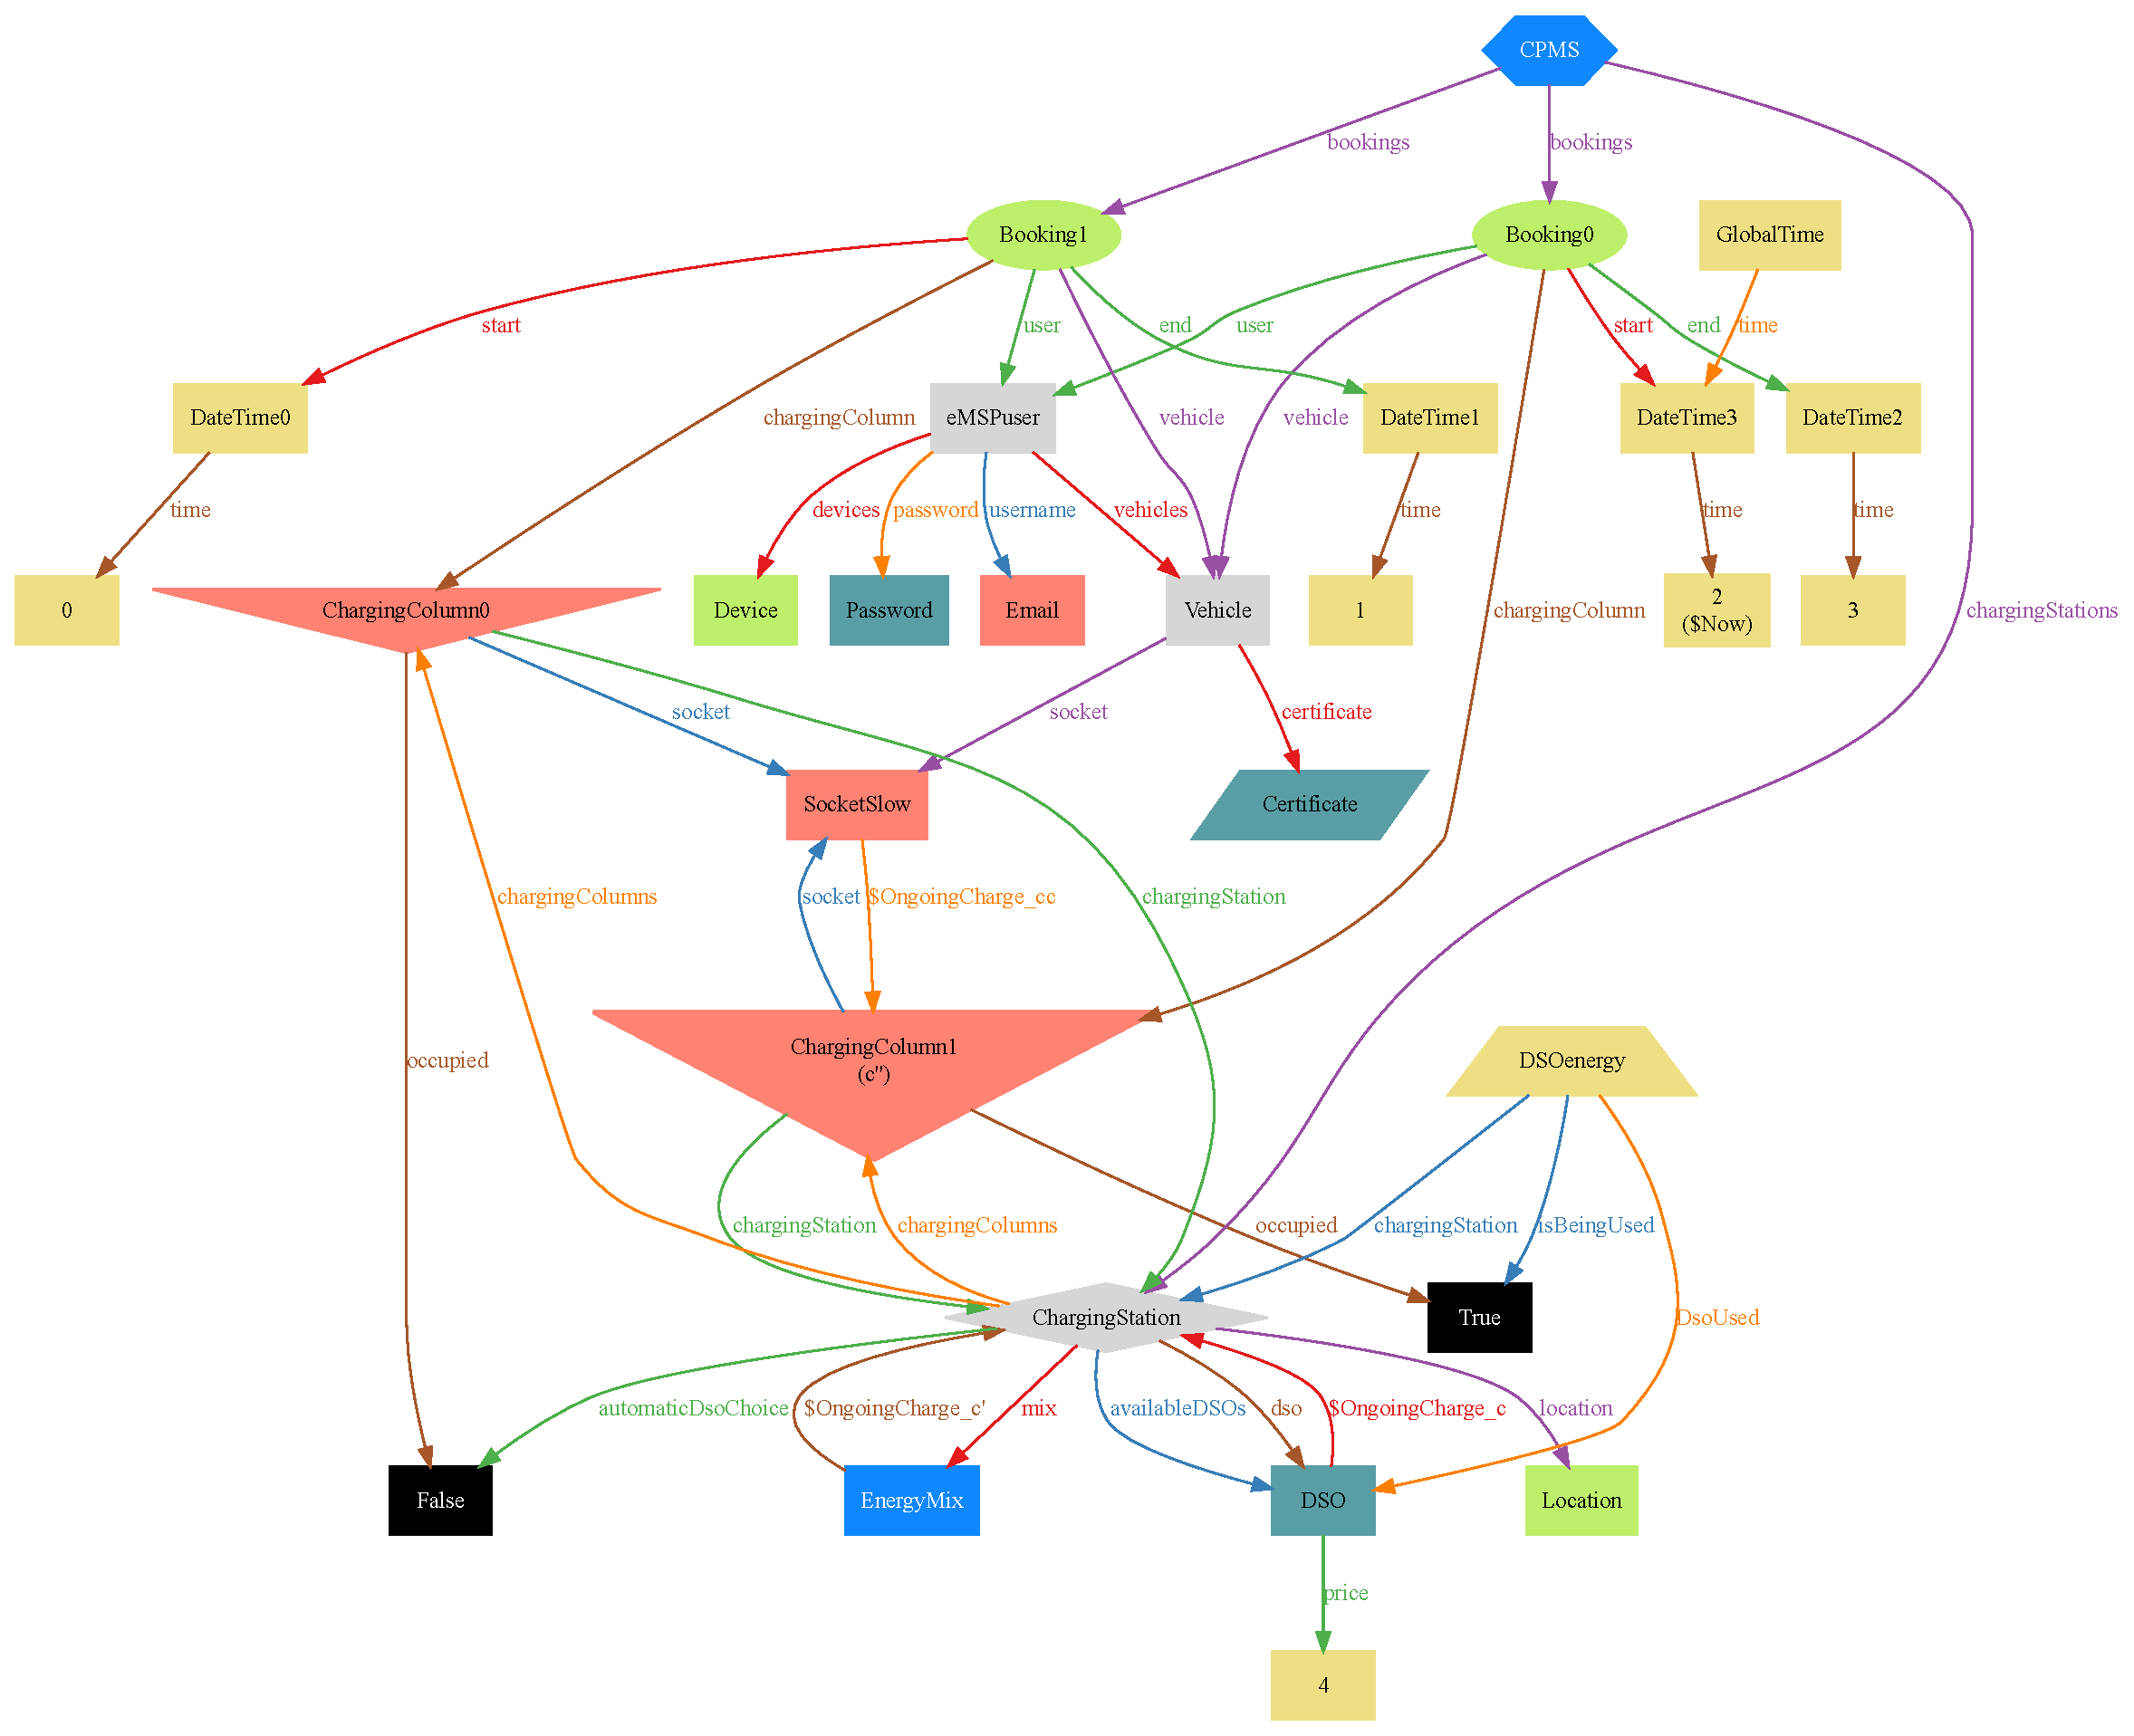
\includegraphics[width=\columnwidth]{./images/alloy/ongoingCharge}
    \caption{the ongoing charge of a vehicle at the charging column.}
\end{figure}

\pagebreak

\subsection{Creation of a booking}

This diagram shows the creation of the first booking by an eMSP user (which is not depicted here) at a specific charging station. The relative column is associated automatically by the system.

\begin{minted}{Alloy}
pred BookCharge[c, c': CPMS, b: Booking] {
    c'.users = c.users
    c'.chargingStations = c.chargingStations
    c'.bookings = c.bookings + b
    #Device = 0
    #ChargingColumn = 1
    #DSO = 1
    #eMSPuser = 1
    #CPMSuser = 0
}
\end{minted}

\begin{figure}[h!]
    \centering
    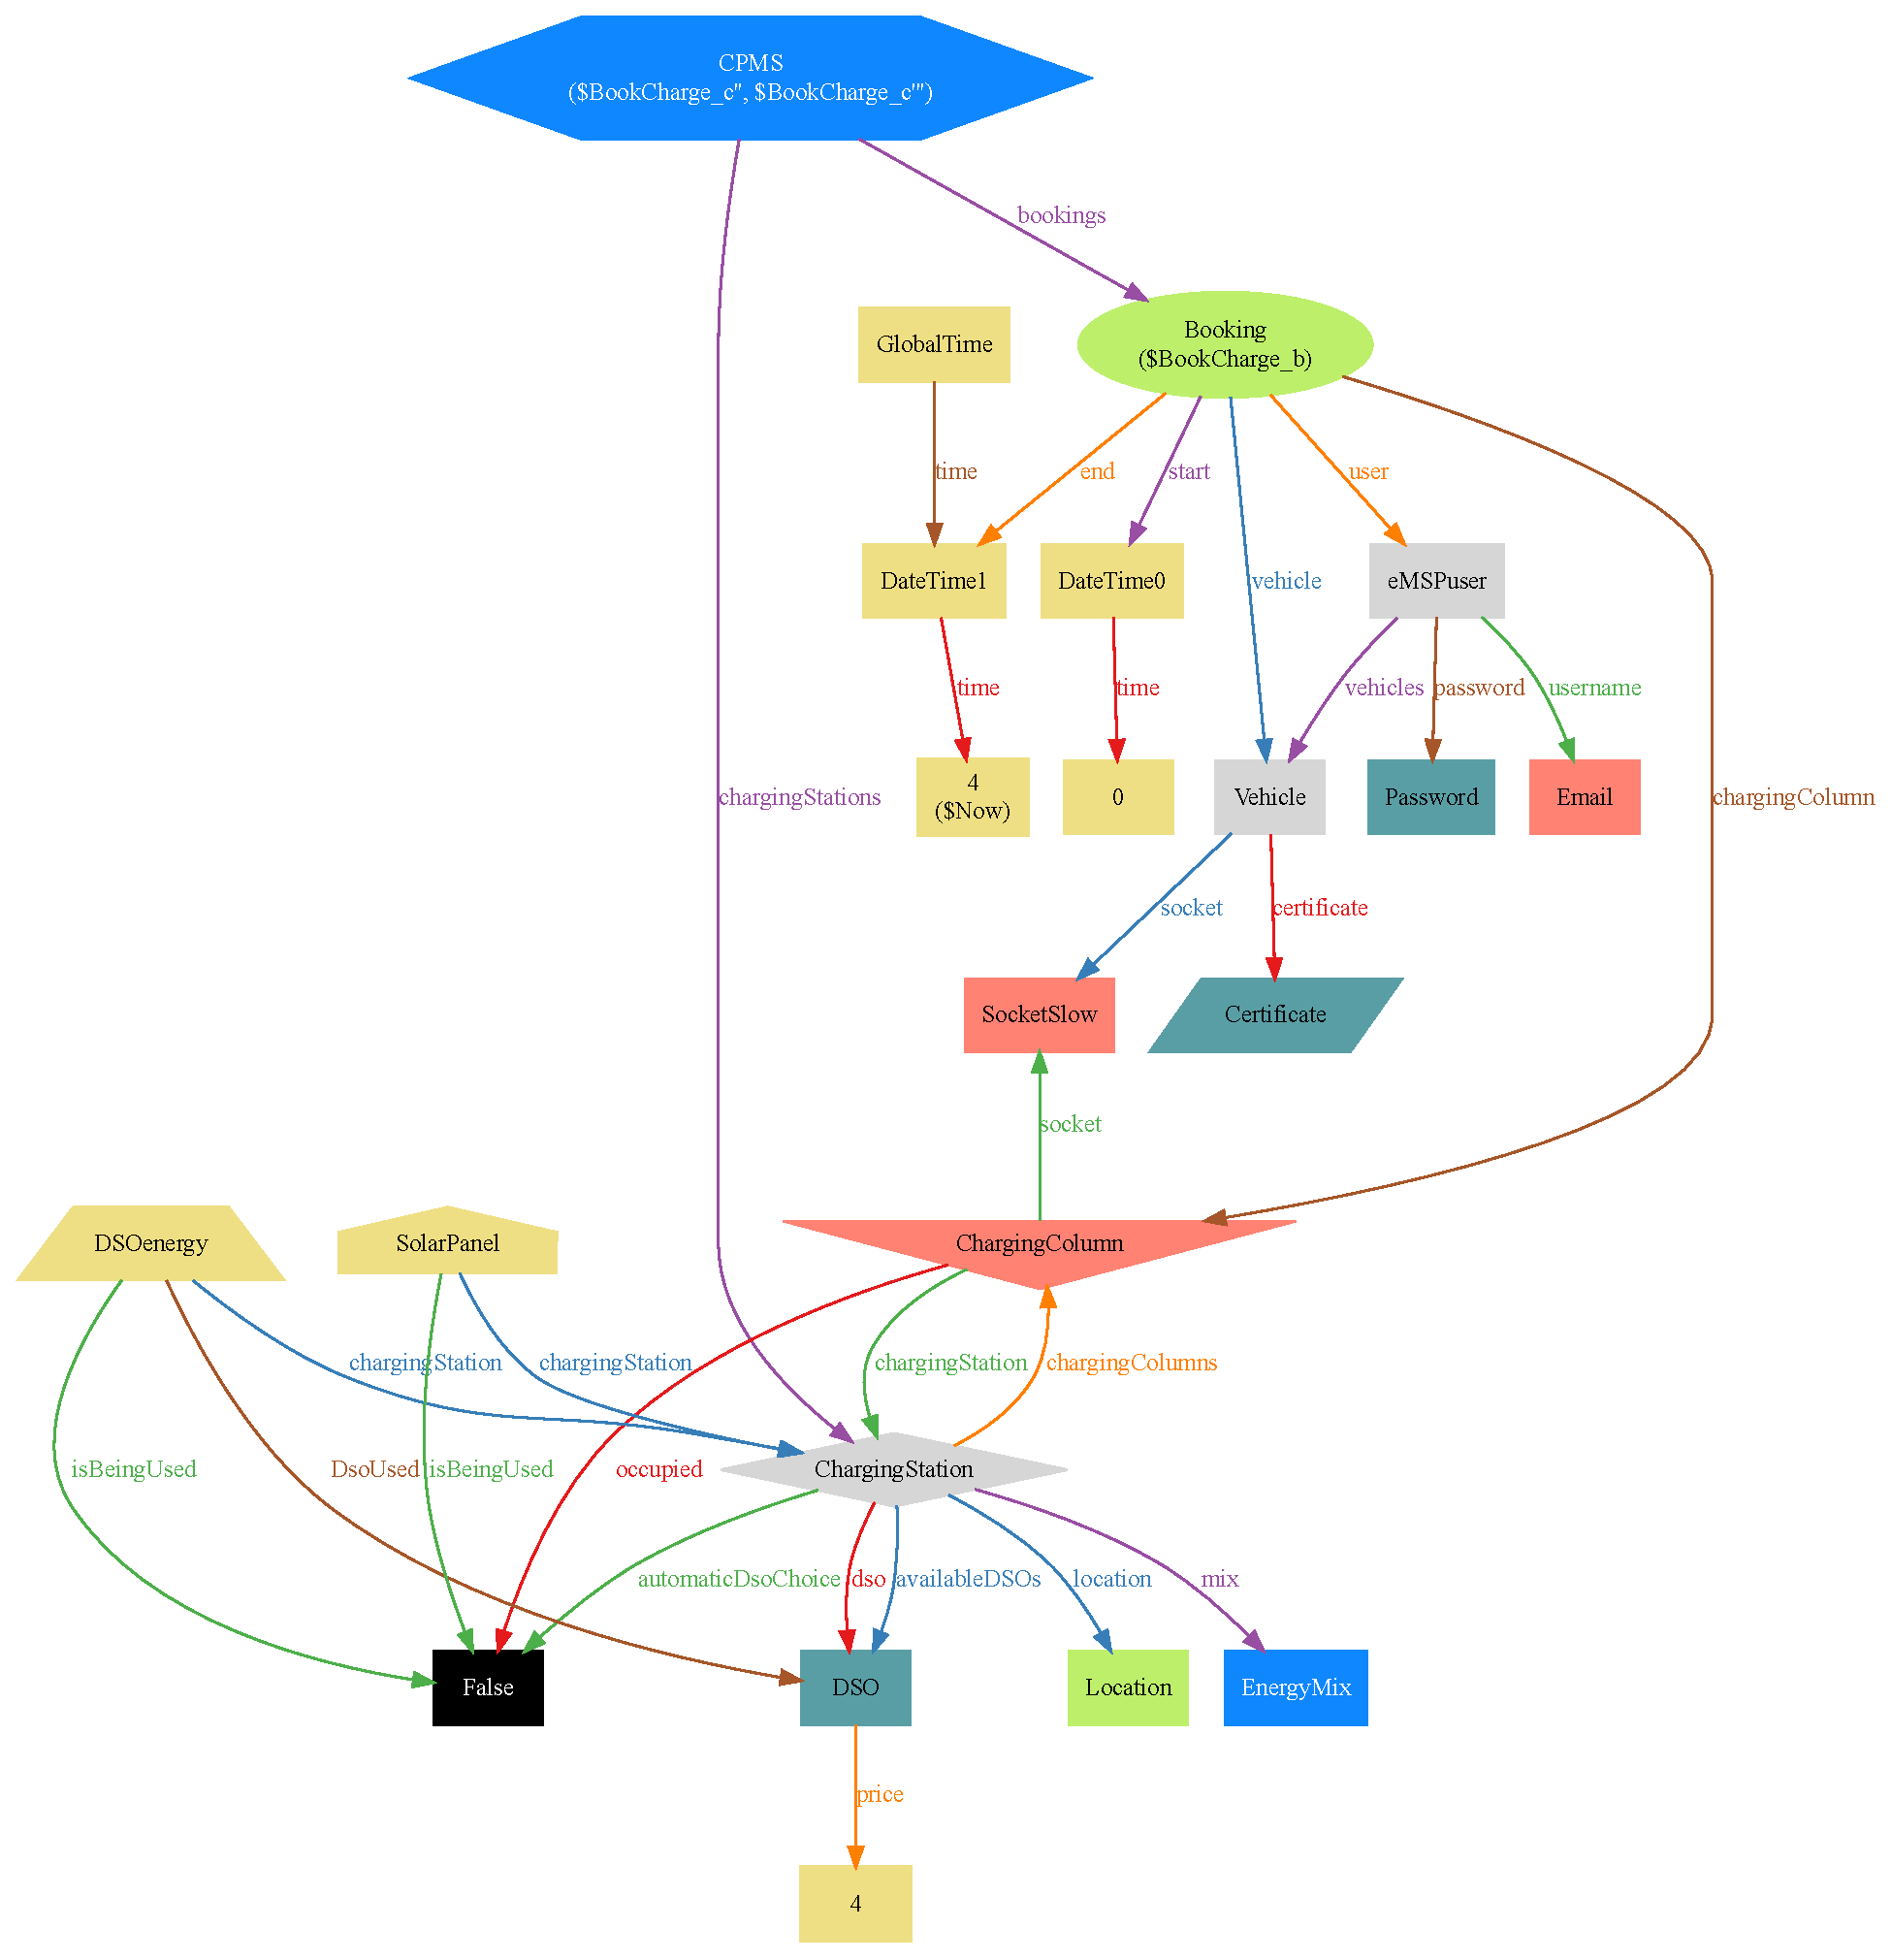
\includegraphics[width=\columnwidth]{./images/alloy/bookCharge}
    \caption{the creation of a new booking.}
\end{figure}

\pagebreak

\subsection{Addition of a vehicle}

This diagram shows the addition of a new vehicle by the eMSP user, connecting it to his account, thus making it available when booking a new charge.

\begin{minted}{Alloy}
pred AddVehicle[u, u': eMSPuser, v: Vehicle] {
    u'.username = u.username
    u'.password = u.password
    u'.devices = u.devices
    u'.vehicles = u.vehicles + v
    u'.favorites = u.favorites
    #GlobalTime = 0
    #CPMS = 0
    #Device = 1
    #Vehicle = 2
}
\end{minted}

\begin{figure}[h!]
    \centering
    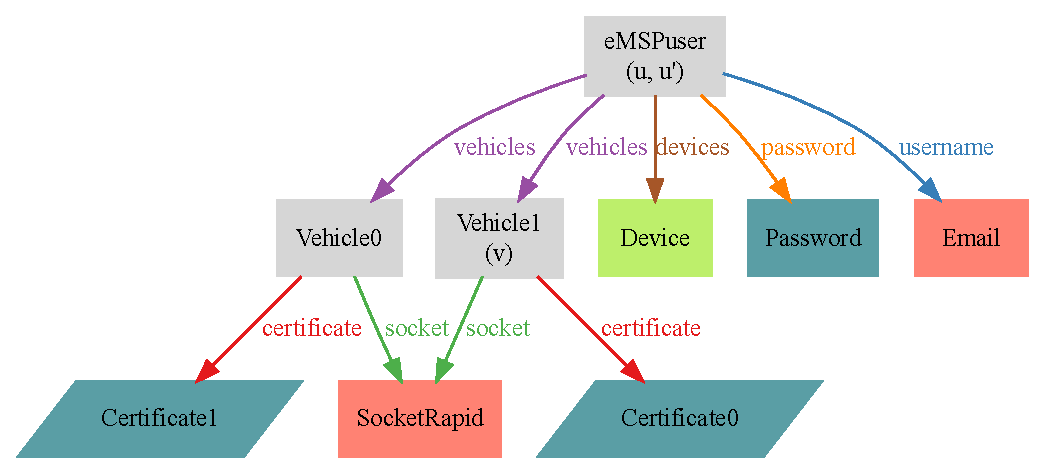
\includegraphics[width=0.5\columnwidth]{./images/alloy/vehicle}
    \caption{the addition of a new vehicle by the eMSP user.}
\end{figure}

\pagebreak

\subsection{Charging station sources}

This diagram shows that a charging station can have multiple energy sources, but that according to the energy mix, some of them may not be used at a specific point in time.

\begin{minted}{Alloy}
pred Sources {
    #eMSPuser = 0
    #CPMS = 1
    #CPMSuser = 0
    #ChargingStation = 1
    #EnergySource = 6
    #GlobalTime = 0
    some d: DSOenergy | d.isBeingUsed = False
}
\end{minted}

\begin{figure}[h!]
    \centering
    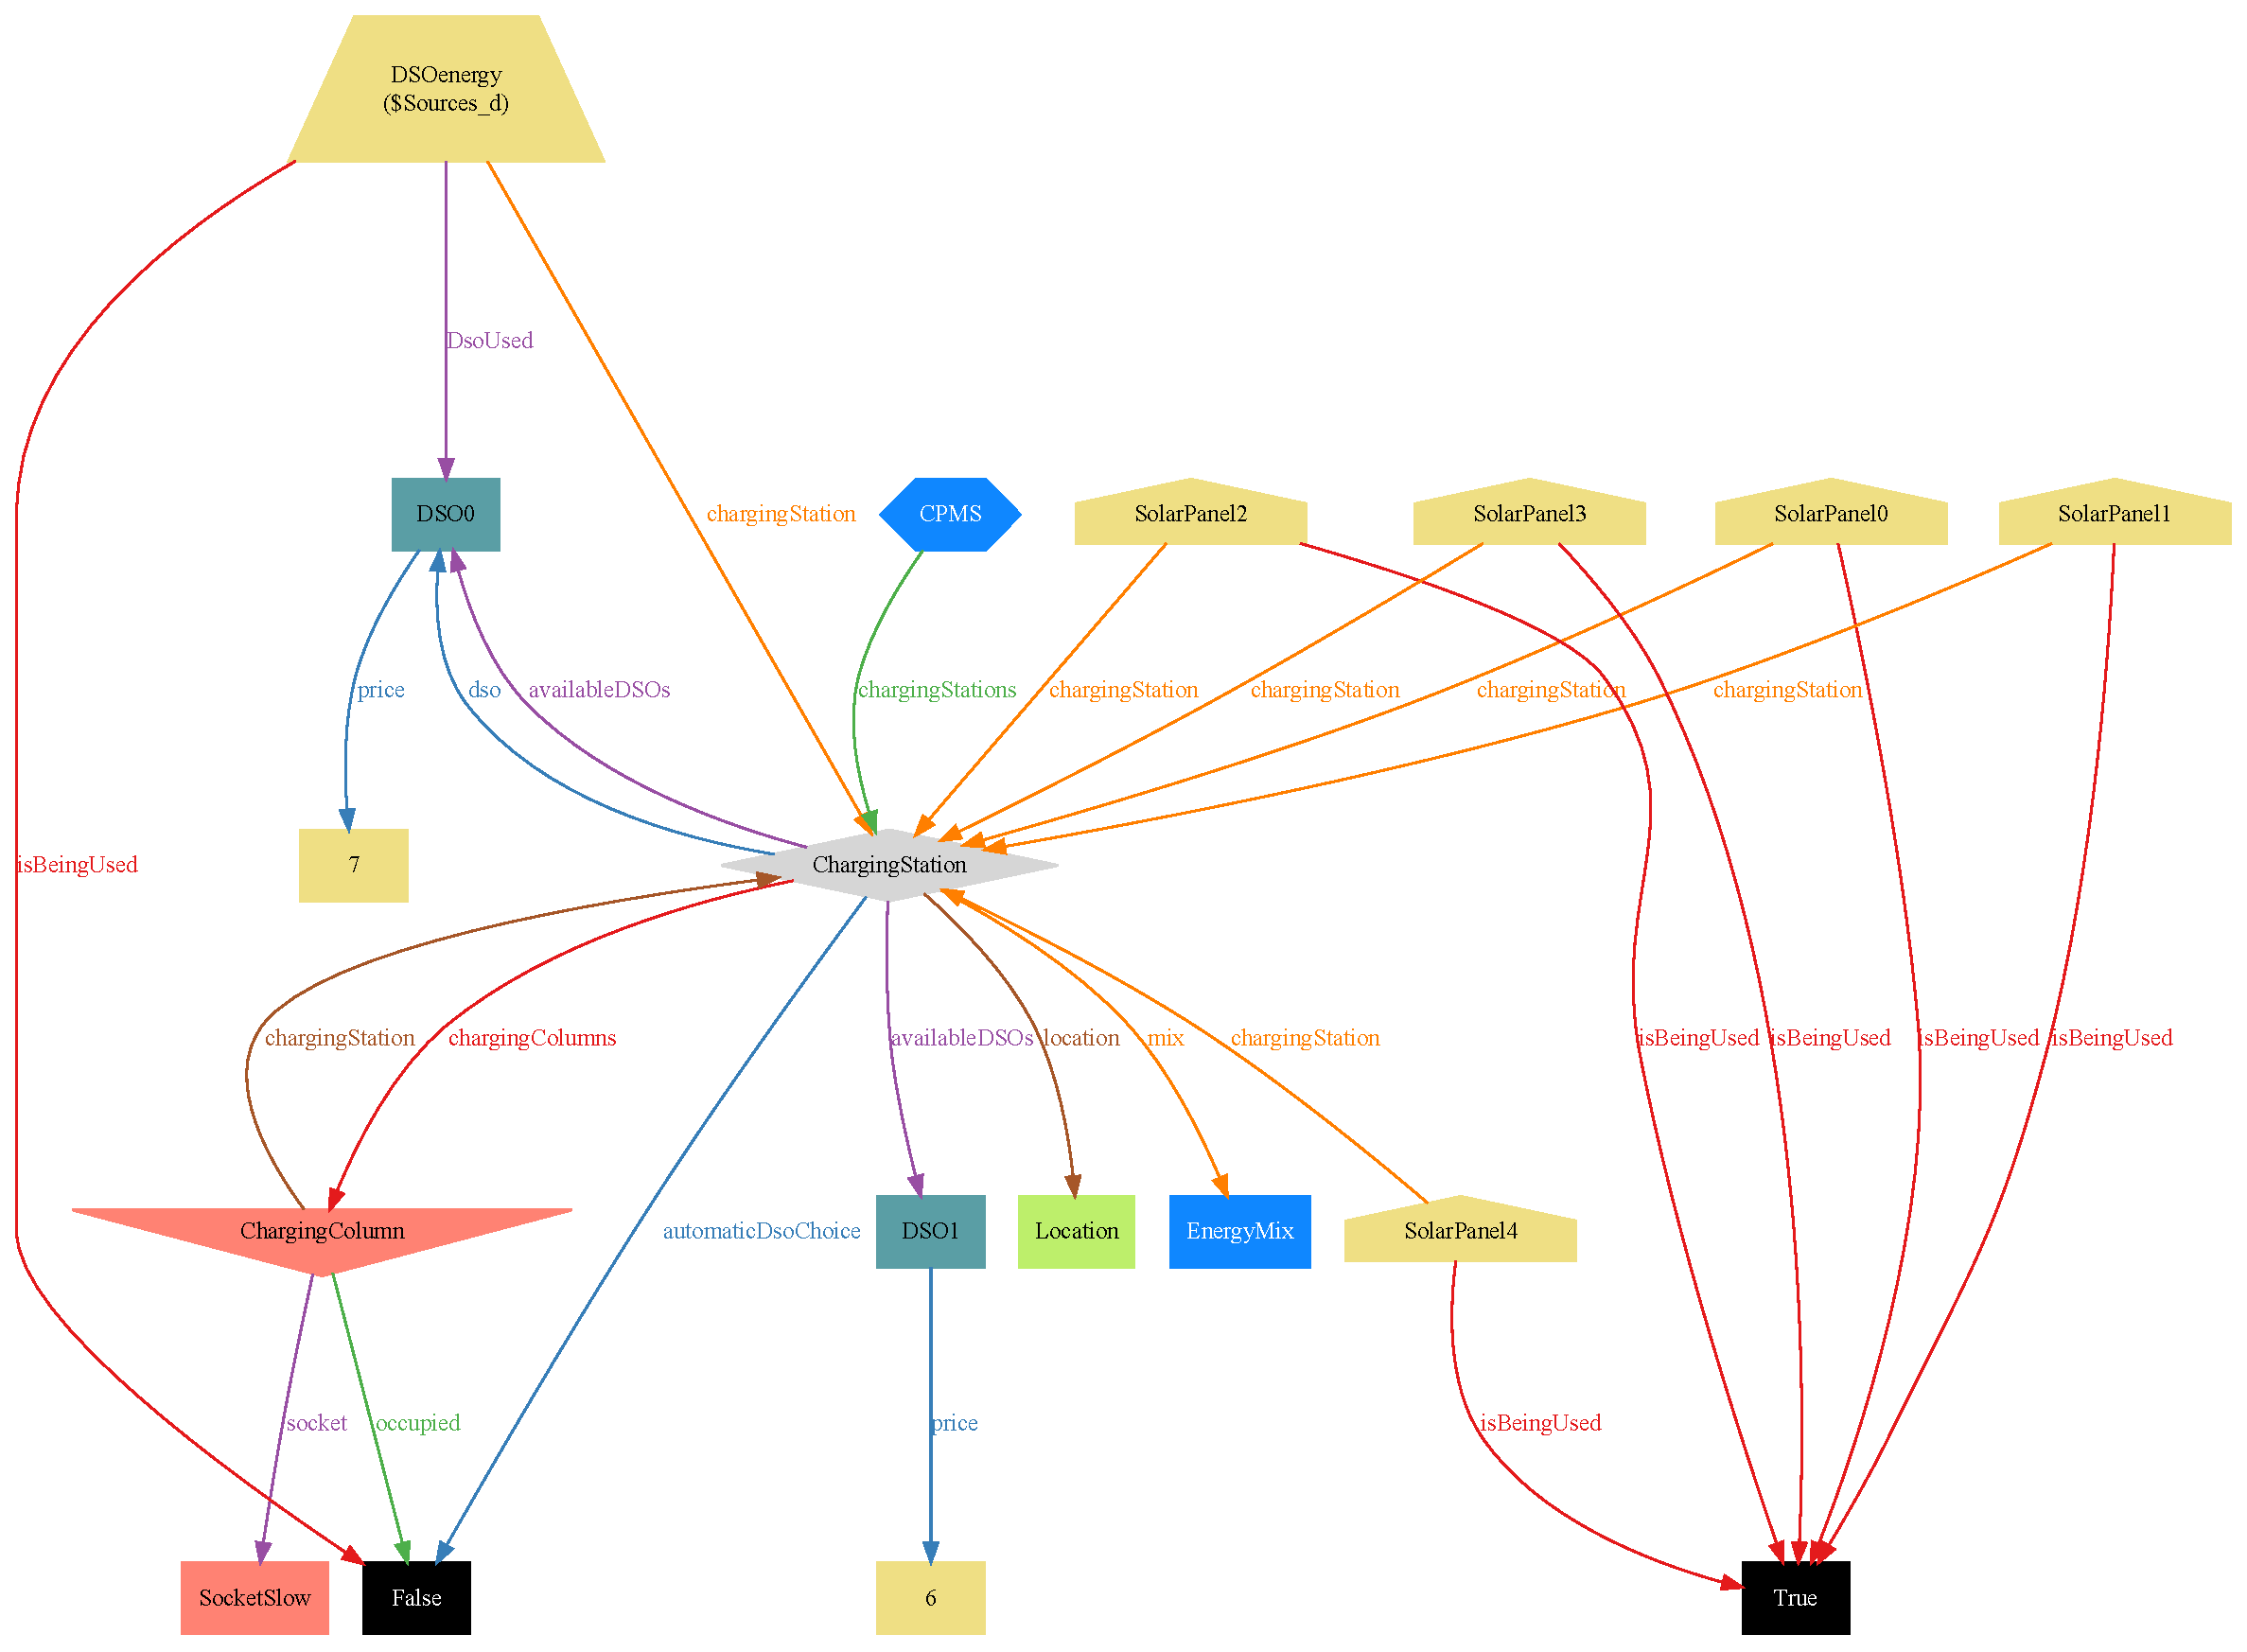
\includegraphics[width=\columnwidth]{./images/alloy/sources}
    \caption{the energetic situation at the charging station.}
\end{figure}

\pagebreak

\subsection{Automatic DSO choice}

This diagram shows the choice of a DSO from which buying the energy for supplying the charging stations which have in their energy mix the energy coming from the DSO.

\begin{minted}{Alloy}
pred AutomaticDSOChoice {
    #ChargingStation = 2
    #DSO > 2
    #eMSPuser = 0
    some cs: ChargingStation | cs.automaticDsoChoice = True
    some cs: ChargingStation | cs.automaticDsoChoice = False
    all cs: ChargingStation | #cs.availableDSOs > 1
}
\end{minted}

\begin{figure}[h!]
    \centering
    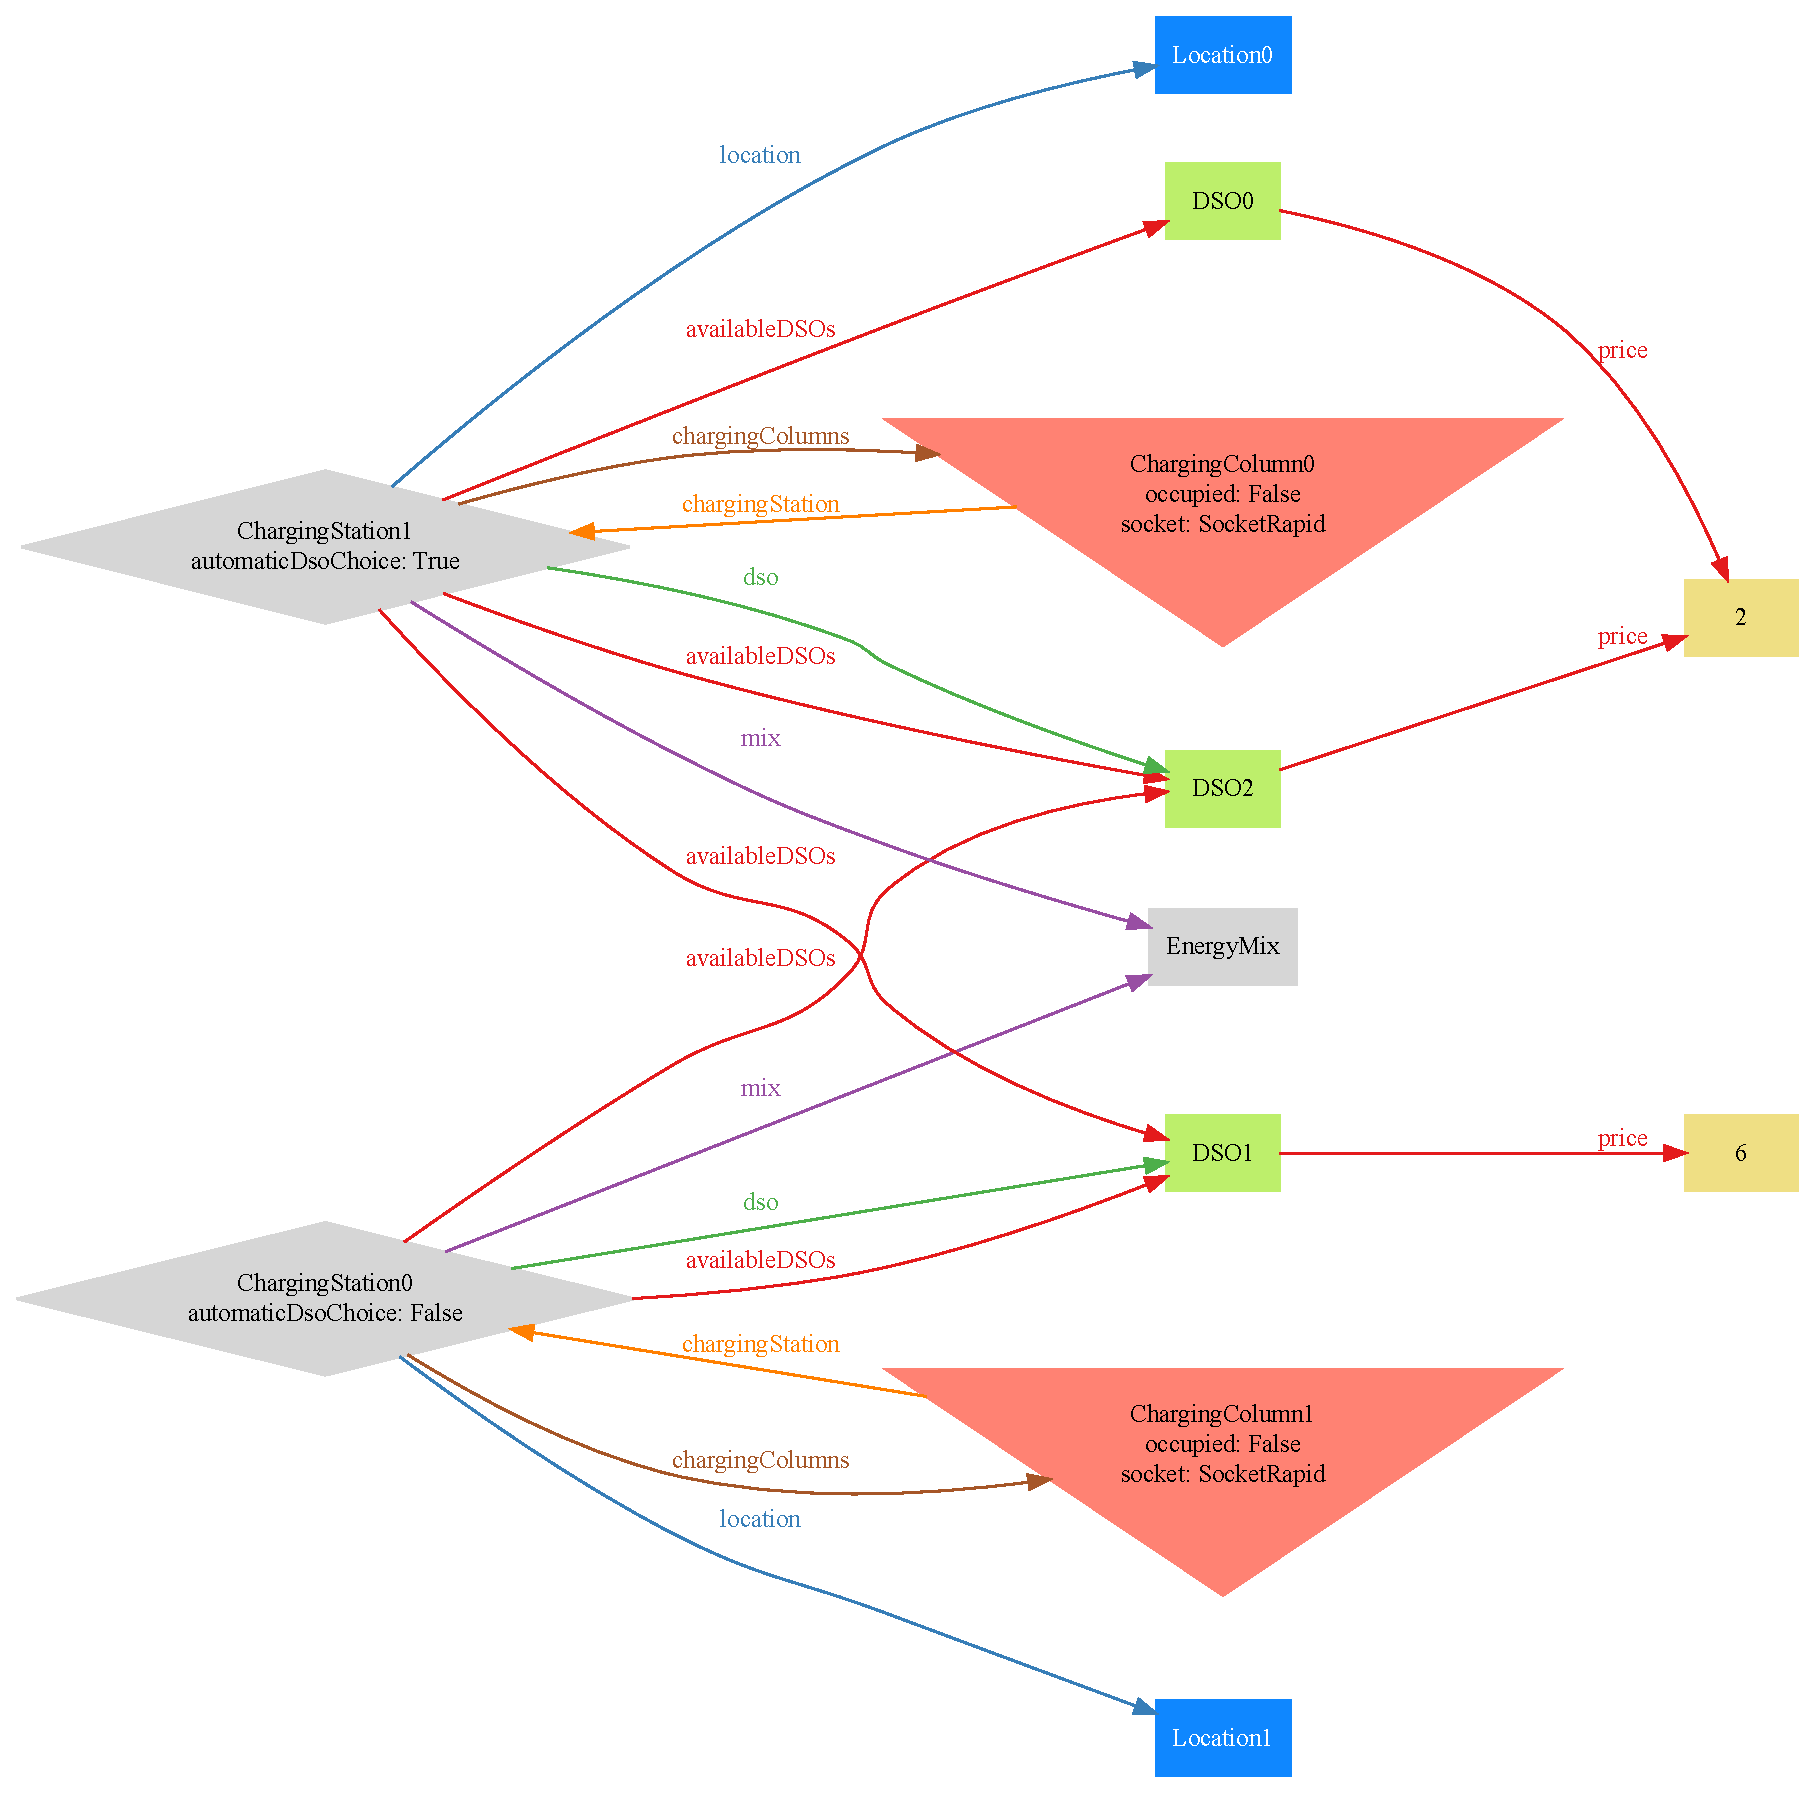
\includegraphics[width=\columnwidth]{./images/alloy/autoDSO}
    \caption{the automatic choice of a DSO.}
\end{figure}

\pagebreak

\subsection{A rather complete world}

This diagram shows a world which tries to be as complete as possible.

\begin{minted}{Alloy}
pred GenericWorld {
    #Email = 3
    #Password = 4
    #eMSPuser = 2
    #Vehicle >= 1
    #Device >= 1
    #CPMS = 1
    #CPMSuser = 2
    #ChargingStation >= 2
    #Booking >= 2
    #DSO >= 2
    #EnergySource >= 3
    no u: eMSPuser | #u.vehicles = 0
    some c: ChargingColumn | c.occupied = True
}
\end{minted}

\begin{figure}[h!]
    \centering
    
\includegraphics[width=\columnwidth]{./images/alloy/generic}
    \caption{a generic, but rather complete, world.}
\end{figure}
